\documentclass[tikz,border=4pt]{standalone}
\usepackage{amsmath,amssymb,bm}
\usepackage{tikz}
\usetikzlibrary{arrows.meta,calc,positioning,fit,backgrounds,decorations.pathreplacing,shapes.geometric,quotes}
\definecolor{okBlue}{HTML}{4472C4}
\definecolor{okRed}{HTML}{C0504D}
\definecolor{okGreen}{HTML}{55A868}
\definecolor{okOrange}{HTML}{D98E04}
\definecolor{okPurple}{HTML}{7E57C2}
\definecolor{okGray}{HTML}{666666}
\definecolor{softBlue}{HTML}{EAF1FB}
\definecolor{softRed}{HTML}{F9ECEB}
\definecolor{softGreen}{HTML}{EDF7F0}
\tikzset{
  >={Latex[length=2.2mm,width=2.0mm]},
  every node/.style={font=\small},
  mathbox/.style={draw=black!55, rounded corners=2pt, very thick, fill=black!2, inner sep=5pt, align=center},
  chip/.style={draw=black!45, rounded corners=1.6pt, fill=black!1, inner sep=2pt, align=center},
  panel/.style={draw=black!55, rounded corners=2pt, line width=0.8pt},
  lightpanel/.style={draw=black!25, rounded corners=2pt, line width=0.5pt},
  flow/.style={-{Latex[length=2.3mm]}, line width=1.0pt, draw=black!70},
  thinflow/.style={-{Latex[length=1.9mm]}, line width=0.8pt, draw=black!55},
  faintcol/.style={draw=black!18, line width=0.6pt},
  reglabel/.style={font=\normalsize},
  srcA/.style={circle, draw=okBlue!70!black, fill=okBlue!15, minimum size=5.2pt, inner sep=0pt},
  srcB/.style={circle, draw=okRed!70!black, fill=okRed!15, minimum size=5.2pt, inner sep=0pt},
  tgtA/.style={circle, draw=okBlue!70!black, fill=okBlue!15, minimum size=5.2pt, inner sep=0pt},
  tgtB/.style={circle, draw=okRed!70!black, fill=okRed!15, minimum size=5.2pt, inner sep=0pt},
  crossdot/.style={diamond, draw=okOrange!80!black, fill=okOrange!85, minimum size=6pt, inner sep=0pt},
  kedge/.style={draw=okBlue!60!black, line width=0.9pt, opacity=0.50},
  triangleedge/.style={draw=okRed!75!black, line width=1.1pt, opacity=0.55},
  matching/.style={draw=okGreen!70!black, line width=1.8pt},
  absent/.style={draw=black!15, dashed, line width=0.55pt},
  qdata/.style={circle, fill=okGreen!75!black, draw=okGreen!55!black, minimum size=4.2pt, inner sep=0pt},
  qx/.style={rectangle, draw=okPurple!85!black, fill=white, minimum size=5.3pt, inner sep=0pt, line width=0.7pt},
  qz/.style={diamond, draw=okOrange!85!black, fill=white, minimum size=5.3pt, inner sep=0pt, line width=0.7pt},
  routeA/.style={draw=okBlue!85!black, line width=1.15pt, line cap=round, line join=round},
  routeB/.style={draw=okRed!85!black, line width=1.15pt, line cap=round, line join=round},
  access/.style={draw=black!40, densely dotted, line width=0.55pt},
  layA/.style={draw=okBlue!55!black, fill=okBlue!10, line width=0.7pt},
  layB/.style={draw=okRed!55!black, fill=okRed!10, line width=0.7pt},
  layBase/.style={draw=black!35, fill=black!5, line width=0.7pt},
  titleline/.style={font=\normalsize\bfseries},
  paneltag/.style={font=\bfseries\normalsize},
}

\begin{document}
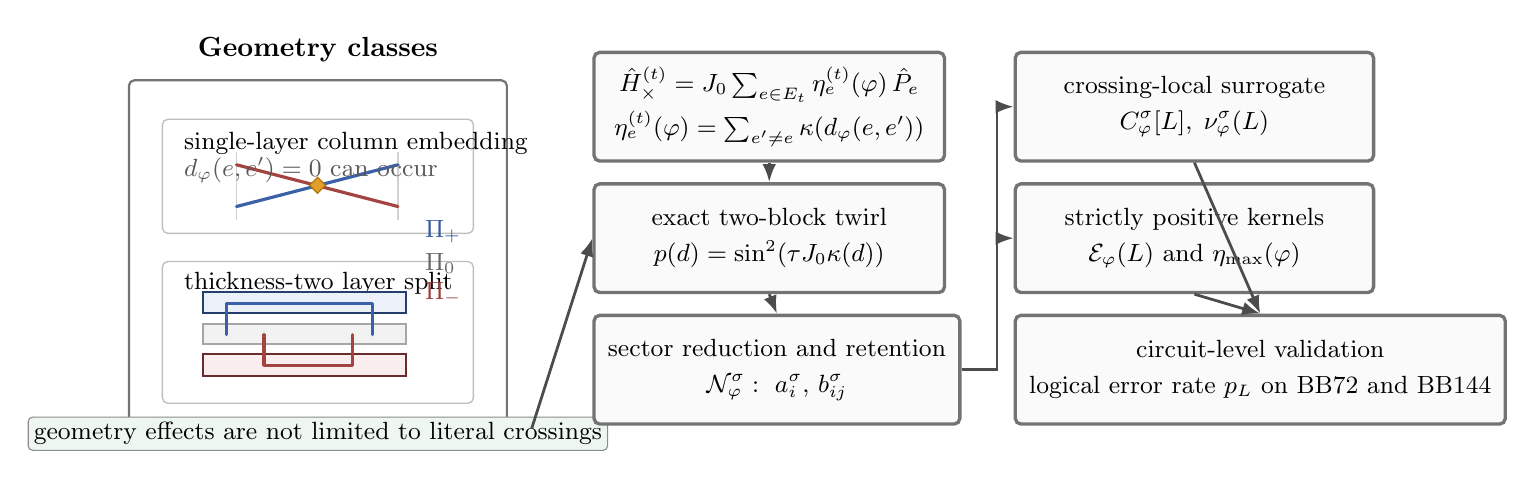
\begin{tikzpicture}[x=1cm,y=1cm]
  % left geometry box
  \node[panel, minimum width=4.8cm, minimum height=4.65cm, anchor=north west] (left) at (0,0) {};
  \node[titleline, anchor=south] at ($(left.north)+(0,0.10)$) {Geometry classes};
  \node[lightpanel, minimum width=3.95cm, minimum height=1.45cm, anchor=north] (m1) at ($(left.north)+(0,-0.50)$) {};
  \node[anchor=west] at ($(m1.west)+(0.16,0.42)$) {single-layer column embedding};
  \foreach \x in {0.95,3.00} {\draw[faintcol] ($(m1.south west)+(\x,0.18)$)--($(m1.north west)+(\x,-0.42)$);}      
  \draw[routeA] ($(m1.south west)+(0.95,0.35)$)--($(m1.south west)+(3.00,0.88)$);
  \draw[routeB] ($(m1.south west)+(0.95,0.88)$)--($(m1.south west)+(3.00,0.35)$);
  \node[crossdot] at ($(m1.south west)+(1.98,0.62)$) {};
  \node[anchor=west, text=black!65] at ($(m1.west)+(0.16,0.08)$) {$d_{\varphi}(e,e')=0$ can occur};

  \node[lightpanel, minimum width=3.95cm, minimum height=1.80cm, anchor=north] (m2) at ($(m1.south)+(0,-0.34)$) {};
  \node[anchor=west] at ($(m2.west)+(0.16,0.62)$) {thickness-two layer split};
  \fill[layA] ($(m2.south west)+(0.52,1.15)$) rectangle ($(m2.south west)+(3.10,1.42)$);
  \fill[layBase] ($(m2.south west)+(0.52,0.76)$) rectangle ($(m2.south west)+(3.10,1.01)$);
  \fill[layB] ($(m2.south west)+(0.52,0.36)$) rectangle ($(m2.south west)+(3.10,0.63)$);
  \draw[routeA] ($(m2.south west)+(0.82,0.88)$)--($(m2.south west)+(0.82,1.28)$)--($(m2.south west)+(2.68,1.28)$)--($(m2.south west)+(2.68,0.88)$);
  \draw[routeB] ($(m2.south west)+(1.30,0.88)$)--($(m2.south west)+(1.30,0.49)$)--($(m2.south west)+(2.42,0.49)$)--($(m2.south west)+(2.42,0.88)$);
  \node[anchor=west, text=okBlue!80!black] at ($(m2.west)+(3.22,1.28)$) {$\Pi_+$};
  \node[anchor=west, text=black!60] at ($(m2.west)+(3.22,0.88)$) {$\Pi_0$};
  \node[anchor=west, text=okRed!80!black] at ($(m2.west)+(3.22,0.49)$) {$\Pi_-$};
  \node[chip, fill=softGreen, anchor=north] at ($(m2.south)+(0,-0.16)$) {geometry effects are not limited to literal crossings};

  % center stack
  \node[mathbox, minimum width=4.45cm, minimum height=1.38cm, anchor=west] (g1) at (5.90,-0.35)
    {$\hat H_{\times}^{(t)}=J_0\sum_{e\in E_t}\eta_e^{(t)}(\varphi)\,\hat P_e$\\[2pt]
     $\eta_e^{(t)}(\varphi)=\sum_{e'\neq e}\kappa\!\left(d_{\varphi}(e,e')\right)$};
  \node[mathbox, minimum width=4.45cm, minimum height=1.38cm, anchor=west] (g2) at (5.90,-2.02)
    {exact two-block twirl\\[2pt]
     $p(d)=\sin^2(\tau J_0\kappa(d))$};
  \node[mathbox, minimum width=4.45cm, minimum height=1.38cm, anchor=west] (g3) at (5.90,-3.69)
    {sector reduction and retention\\[2pt]
     $\mathcal N_{\varphi}^{\sigma}:\ a_i^{\sigma},\, b_{ij}^{\sigma}$};
  \draw[flow] ($(left.east)+(0.30,-2.10)$) -- (g2.west);
  \draw[flow] (g1.south) -- (g2.north);
  \draw[flow] (g2.south) -- (g3.north);

  % right stack
  \node[mathbox, minimum width=4.55cm, minimum height=1.38cm, anchor=west] (h1) at (11.25,-0.35)
    {crossing-local surrogate\\[2pt]
     $C_{\varphi}^{\sigma}[L],\; \nu_{\varphi}^{\sigma}(L)$};
  \node[mathbox, minimum width=4.55cm, minimum height=1.38cm, anchor=west] (h2) at (11.25,-2.02)
    {strictly positive kernels\\[2pt]
     $\mathcal E_{\varphi}(L)$ and $\eta_{\max}(\varphi)$};
  \node[mathbox, minimum width=4.55cm, minimum height=1.38cm, anchor=west] (h3) at (11.25,-3.69)
    {circuit-level validation\\[2pt]
     logical error rate $p_L$ on BB72 and BB144};
  \draw[flow] (g3.east) -- ++(0.45,0) |- (h1.west);
  \draw[flow] (g3.east) -- ++(0.45,0) |- (h2.west);
  \draw[flow] (h1.south) -- (h3.north);
  \draw[flow] (h2.south) -- (h3.north);
\end{tikzpicture}
\end{document}
